% FFT butterfly diagram, n = 8, bit-reversed inputs. Generated by a short script.
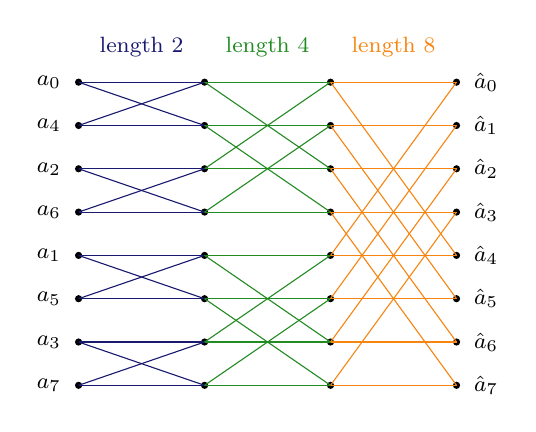
\begin{tikzpicture}[every node/.style={font=\footnotesize}]
\fill (0.00,0.00) circle (1.3pt);
\fill (0.00,-0.55) circle (1.3pt);
\fill (0.00,-1.10) circle (1.3pt);
\fill (0.00,-1.65) circle (1.3pt);
\fill (0.00,-2.20) circle (1.3pt);
\fill (0.00,-2.75) circle (1.3pt);
\fill (0.00,-3.30) circle (1.3pt);
\fill (0.00,-3.85) circle (1.3pt);
\fill (1.60,0.00) circle (1.3pt);
\fill (1.60,-0.55) circle (1.3pt);
\fill (1.60,-1.10) circle (1.3pt);
\fill (1.60,-1.65) circle (1.3pt);
\fill (1.60,-2.20) circle (1.3pt);
\fill (1.60,-2.75) circle (1.3pt);
\fill (1.60,-3.30) circle (1.3pt);
\fill (1.60,-3.85) circle (1.3pt);
\fill (3.20,0.00) circle (1.3pt);
\fill (3.20,-0.55) circle (1.3pt);
\fill (3.20,-1.10) circle (1.3pt);
\fill (3.20,-1.65) circle (1.3pt);
\fill (3.20,-2.20) circle (1.3pt);
\fill (3.20,-2.75) circle (1.3pt);
\fill (3.20,-3.30) circle (1.3pt);
\fill (3.20,-3.85) circle (1.3pt);
\fill (4.80,0.00) circle (1.3pt);
\fill (4.80,-0.55) circle (1.3pt);
\fill (4.80,-1.10) circle (1.3pt);
\fill (4.80,-1.65) circle (1.3pt);
\fill (4.80,-2.20) circle (1.3pt);
\fill (4.80,-2.75) circle (1.3pt);
\fill (4.80,-3.30) circle (1.3pt);
\fill (4.80,-3.85) circle (1.3pt);
\node[left] at (-0.1,0.00) {$a_0$};
\node[right] at (4.90,0.00) {$\hat a_0$};
\node[left] at (-0.1,-0.55) {$a_4$};
\node[right] at (4.90,-0.55) {$\hat a_1$};
\node[left] at (-0.1,-1.10) {$a_2$};
\node[right] at (4.90,-1.10) {$\hat a_2$};
\node[left] at (-0.1,-1.65) {$a_6$};
\node[right] at (4.90,-1.65) {$\hat a_3$};
\node[left] at (-0.1,-2.20) {$a_1$};
\node[right] at (4.90,-2.20) {$\hat a_4$};
\node[left] at (-0.1,-2.75) {$a_5$};
\node[right] at (4.90,-2.75) {$\hat a_5$};
\node[left] at (-0.1,-3.30) {$a_3$};
\node[right] at (4.90,-3.30) {$\hat a_6$};
\node[left] at (-0.1,-3.85) {$a_7$};
\node[right] at (4.90,-3.85) {$\hat a_7$};
\draw[MidnightBlue] (0.00,0.00)--(1.60,0.00);
\draw[MidnightBlue] (0.00,-0.55)--(1.60,0.00);
\draw[MidnightBlue] (0.00,-0.55)--(1.60,-0.55);
\draw[MidnightBlue] (0.00,0.00)--(1.60,-0.55);
\draw[MidnightBlue] (0.00,-1.10)--(1.60,-1.10);
\draw[MidnightBlue] (0.00,-1.65)--(1.60,-1.10);
\draw[MidnightBlue] (0.00,-1.65)--(1.60,-1.65);
\draw[MidnightBlue] (0.00,-1.10)--(1.60,-1.65);
\draw[MidnightBlue] (0.00,-2.20)--(1.60,-2.20);
\draw[MidnightBlue] (0.00,-2.75)--(1.60,-2.20);
\draw[MidnightBlue] (0.00,-2.75)--(1.60,-2.75);
\draw[MidnightBlue] (0.00,-2.20)--(1.60,-2.75);
\draw[MidnightBlue] (0.00,-3.30)--(1.60,-3.30);
\draw[MidnightBlue] (0.00,-3.85)--(1.60,-3.30);
\draw[MidnightBlue] (0.00,-3.85)--(1.60,-3.85);
\draw[MidnightBlue] (0.00,-3.30)--(1.60,-3.85);
\draw[ForestGreen] (1.60,0.00)--(3.20,0.00);
\draw[ForestGreen] (1.60,-1.10)--(3.20,0.00);
\draw[ForestGreen] (1.60,-0.55)--(3.20,-0.55);
\draw[ForestGreen] (1.60,-1.65)--(3.20,-0.55);
\draw[ForestGreen] (1.60,-1.10)--(3.20,-1.10);
\draw[ForestGreen] (1.60,0.00)--(3.20,-1.10);
\draw[ForestGreen] (1.60,-1.65)--(3.20,-1.65);
\draw[ForestGreen] (1.60,-0.55)--(3.20,-1.65);
\draw[ForestGreen] (1.60,-2.20)--(3.20,-2.20);
\draw[ForestGreen] (1.60,-3.30)--(3.20,-2.20);
\draw[ForestGreen] (1.60,-2.75)--(3.20,-2.75);
\draw[ForestGreen] (1.60,-3.85)--(3.20,-2.75);
\draw[ForestGreen] (1.60,-3.30)--(3.20,-3.30);
\draw[ForestGreen] (1.60,-2.20)--(3.20,-3.30);
\draw[ForestGreen] (1.60,-3.85)--(3.20,-3.85);
\draw[ForestGreen] (1.60,-2.75)--(3.20,-3.85);
\draw[BurntOrange] (3.20,0.00)--(4.80,0.00);
\draw[BurntOrange] (3.20,-2.20)--(4.80,0.00);
\draw[BurntOrange] (3.20,-0.55)--(4.80,-0.55);
\draw[BurntOrange] (3.20,-2.75)--(4.80,-0.55);
\draw[BurntOrange] (3.20,-1.10)--(4.80,-1.10);
\draw[BurntOrange] (3.20,-3.30)--(4.80,-1.10);
\draw[BurntOrange] (3.20,-1.65)--(4.80,-1.65);
\draw[BurntOrange] (3.20,-3.85)--(4.80,-1.65);
\draw[BurntOrange] (3.20,-2.20)--(4.80,-2.20);
\draw[BurntOrange] (3.20,0.00)--(4.80,-2.20);
\draw[BurntOrange] (3.20,-2.75)--(4.80,-2.75);
\draw[BurntOrange] (3.20,-0.55)--(4.80,-2.75);
\draw[BurntOrange] (3.20,-3.30)--(4.80,-3.30);
\draw[BurntOrange] (3.20,-1.10)--(4.80,-3.30);
\draw[BurntOrange] (3.20,-3.85)--(4.80,-3.85);
\draw[BurntOrange] (3.20,-1.65)--(4.80,-3.85);
\node[MidnightBlue] at (0.80,0.45) {length 2};
\node[ForestGreen] at (2.40,0.45) {length 4};
\node[BurntOrange] at (4.00,0.45) {length 8};
\end{tikzpicture}
